\documentclass{beamer}
\usetheme{Warsaw}

%% Page numbering
\defbeamertemplate*{footline}{shadow theme}{%
\leavevmode%
\hbox{\begin{beamercolorbox}[wd=.5\paperwidth,ht=2.5ex,dp=1.125ex,leftskip=.3cm plus1fil,rightskip=.3cm]{author in head/foot}%
    \usebeamerfont{author in head/foot}\hfill\insertshortauthor
\end{beamercolorbox}%
\begin{beamercolorbox}[wd=.4\paperwidth,ht=2.5ex,dp=1.125ex,leftskip=.3cm,rightskip=.3cm plus1fil]{title in head/foot}%
    \usebeamerfont{title in head/foot}\insertshorttitle\hfill%
\end{beamercolorbox}%
\begin{beamercolorbox}[wd=.1\paperwidth,ht=2.5ex,dp=1.125ex,leftskip=.3cm,rightskip=.3cm plus1fil]{title in head/foot}%
\hfill\insertframenumber\,/\,\inserttotalframenumber
\end{beamercolorbox}}%
\vskip0pt%
}


\usepackage[utf8]{inputenc}
\usepackage[english]{babel}
\usepackage{amsmath}
\usepackage{amsfonts}
\usepackage{amssymb}
\usepackage{graphicx}
\setbeamercovered{invisible} 

\usepackage{pifont}
\newcommand{\cmark}{\ding{51}}%

\hypersetup{bookmarksopen=true,bookmarksopenlevel=4}
\setcounter{tocdepth}{3}

%Information to be included in the title page:
\title{POSOS: Predict the expected answer}
\author{Romain Vial}
\institute{romain.vial@mines-paristech.fr}
\date{Collège de France, April 2018}
 
\begin{document}
 
\frame{\titlepage}

\begin{frame}
\frametitle{Table of Contents}
\tableofcontents[subsubsectionstyle=hide, subsectionstyle=hide]
\end{frame}

\section{Introduction}

\begin{frame}
\frametitle{Introduction}

\centering

\includegraphics[width=.3\linewidth]{images/posos}

Drug misuse could be responsible for more than 144,000 hospitalizations every year in France!

\end{frame}

\begin{frame}
\frametitle{Introduction}
People often ask questions about the drugs they use. How to accurately understand the underlying intent? (contraindication, side effects,...)

\end{frame}

\begin{frame}
\frametitle{Introduction}
Goal: predict the intent associated to a given question among 51 possible categories

\end{frame}

\section{Data Exploration}

\begin{frame}
\frametitle{Dataset}

\begin{itemize}
\item 10,063 questions: 8028 for training, 2035 for testing. 
\item Training set divided in two splits: 80\% training, 20\% validation 
\end{itemize}

\end{frame}

\subsection{Class Imbalance}

\begin{frame}
\frametitle{Class Imbalance}

\centering
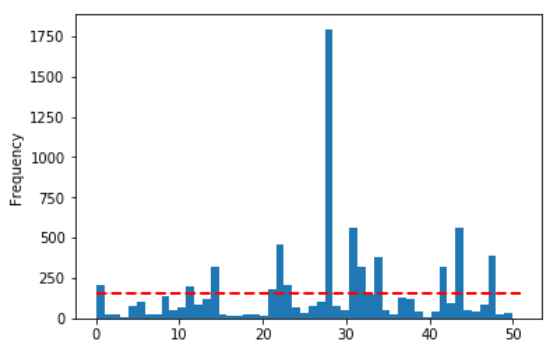
\includegraphics[width=0.7\linewidth]{images/intent_hist}

Class \texttt{28} accounts for 22\% while +30 classes account for $<$1\% each

\end{frame}

\subsection{Dealing with Drug Names}

\begin{frame}
\frametitle{Dealing with Drug Names}

``Par quoi remplacer Aerius et Doliprane ?":
\begin{itemize}
\item ``Par quoi remplacer Aerius et Doliprane ?" + $[2]$
\uncover<2-3>{\item ``Par quoi remplacer $<$MED$>$ et $<$MED$>$ ?"}
\uncover<3>{\item ``Par quoi remplacer $<$MED0$>$ et $<$MED1$>$ ?"}
\end{itemize}

\end{frame}

\section{Proposed Approach}

\subsection{Data Representation}

\begin{frame}
\frametitle{TF-IDF}

\end{frame}

\begin{frame}
\frametitle{Doc2Vec \cite{le2014distributed}}

\end{frame}

\subsection{Classifiers}

\begin{frame}
\frametitle{Support Vector Machine \cite{Cortes1995}}

\end{frame}

\begin{frame}
\frametitle{Xgboost \cite{chen2016xgboost}}

\end{frame}

\begin{frame}
\frametitle{Ensembling}

\end{frame}

\section{Experiments}

\subsection{Quantitative Experiments}

\begin{frame}
\frametitle{Quantitative Experiments}

\centering
\begin{tabular}{|c|c||c|c||c|c|}
\hline
tf-idf & Doc2Vec & SVM & XGB & train & val\\
\hline
\hline
\cmark & & \cmark & & 99.41 & 65.91 \\
\hline
\cmark & & & \cmark & 94.11 & 60.50 \\
\hline
\cmark & & \cmark & \cmark & 99.37 & \textbf{66.71} \\
\hline
\hline
& \cmark & \cmark & & 84.28 & 51.84 \\
\hline
& \cmark & & \cmark & 98.65 & 50.18 \\
\hline
& \cmark & \cmark & \cmark & 93.98 & 52.03 \\
\hline
\end{tabular}
\\~\\
Accuracy of 68.60\% (8/19) on the test set with tf-idf and SVM/XBF ensemble

\end{frame}

\subsection{Qualitative Experiments}

\begin{frame}
\frametitle{Qualitative Experiments}

\centering
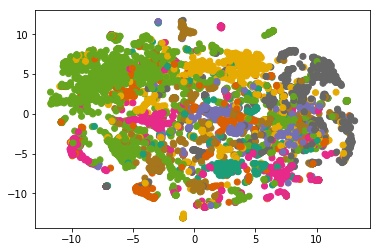
\includegraphics[width=.7\linewidth]{images/embedding}

T-SNE representation of the 50-dimensional Doc2Vec embedding of the training split.

\end{frame}

\section{Conclusion}

\begin{frame}
\frametitle{Conclusion}

\begin{itemize}
\item Improve spelling normalization with e.g.~noisy channel approaches \cite{kernighan1990spelling}
\uncover<2-3>{\item Drug embedding by looking at the co-occurrence matrix}
\uncover<3>{\item Exploring CNN and RNN as a powerful way to learn the features}
\end{itemize}

\end{frame}

\section*{References}

\begin{frame}
\frametitle{References}
{\tiny
\bibliographystyle{apalike}
\bibliography{egbib}}
\end{frame}
 
\end{document}

